\documentclass[11pt,letterpaper]{article}
\usepackage{graphicx, geometry, amsmath, amssymb, hyperref, natbib, booktabs, xcolor, listings, url}
\geometry{margin=1in}
\hypersetup{colorlinks=true, linkcolor=black, citecolor=black, urlcolor=black}

\title{Conformal Admission Control for Overloaded Request Queues}
\author{}
\date{}

\begin{document}
\maketitle

\begin{abstract}
Overloaded request-serving systems must decide, for every arriving request, whether to admit it now without knowing in advance which admissions will later violate a latency service-level objective (SLO). Existing admission-control paradigms either assume a distributional model of traffic and service time (queueing-theoretic, index-based policies) or adapt empirically with no formal safety guarantee (reinforcement-learning controllers). We test a third paradigm: repointing Adaptive Conformal Inference, an online, distribution-free threshold-tracking rule from the conformal prediction literature, directly at the admit/reject decision, so a single scalar threshold updated after every observed outcome tracks a target SLO-violation rate with a finite-sample guarantee and no distributional assumption. We state this guarantee as an explicit theorem in the admission-control setting's own notation, including the precondition that the bound is over admitted requests rather than raw arrivals. We evaluate the resulting policy against a frozen fixed threshold, a misspecified queueing-index policy, a frozen reinforcement-learning-style controller, and a hindsight-optimal oracle on a 210,000-request dataset built from real Azure Functions traces across five traffic regimes, closing a self-referential-evaluation gap from an earlier iteration of this study that had relied on a self-generated traffic simulator. The central finding is structural rather than purely a win for the proposed policy: a single global violation-rate target is only a fair test of any admission policy in regimes where the traffic's natural violation rate is not already far from that target -- even a hindsight-optimal oracle fails a fixed tolerance criterion in regimes whose natural rate sits well below the target, since there is nothing left for an admission policy to correct. In the regimes where the target is a genuine constraint, the conformal controller is the only non-oracle policy within the pre-registered tolerance under sustained drift, and is significantly closer to the target than a frozen reinforcement-learning-style baseline under an adversarially constructed traffic sequence, while remaining statistically indistinguishable from a well-tuned fixed threshold at matched safety. A value-aware admission layer built on the same eligibility set shows no statistically significant value gain over first-come-first-served admission on the real trace, a result we report as a genuine negative finding rather than smoothing it over.
\end{abstract}

\section{Introduction}

Overloaded request-serving systems -- a serverless function platform, a database connection pool, an API gateway in front of a microservice fleet -- must decide, for every incoming request, whether to admit it now or reject it before it consumes resources it cannot repay. This decision is an admission-control problem: choose a subset of arriving requests to serve so that the fraction of admitted requests that miss a latency service-level objective (SLO), such as a P99 response-time target, stays at or below an operator-chosen rate $\alpha$, while admitting as much useful work as possible.

Getting this right matters wherever load is unpredictable and the cost of guessing wrong is real. A function-as-a-service platform processes invocations with wildly different, non-stationary demand across its functions; a single deployment, a viral event, or a shift in a co-located tenant's workload can change the traffic an admission controller sees within minutes. An operator with no bound on the SLO-violation rate either over-provisions to survive worst-case bursts, wasting capacity most of the time, or under-provisions and risks a violation cascade that a single bad five minutes of traffic can trigger. The evaluation in this paper targets that narrower, concrete setting -- a single shared queue or endpoint class governed by one admission threshold -- rather than a claim about coordinated guarantees across a whole multi-tenant fleet; extending the mechanism to per-function or per-tenant thresholds under a joint budget is future work, discussed at the end of this paper.

The problem is hard because the traffic and service-time processes that determine whether a given admission decision will violate an SLO are not known in advance, are rarely stationary, and can change abruptly. Any policy whose safety argument rests on a fitted model of that process is only as safe as the model's fit to the traffic that actually arrives, and the traffic that breaks the fit is exactly the traffic an operator most needs protection from.

The two paradigms in use today accept this fragility as the price of a formal argument, or drop the formal argument entirely. Queueing-theoretic and index-based controllers, including the classical Whittle-index construction for restless-bandit admission control \citep{Whittle1988} and its birth-death-model extension to queueing admission \citep{NinoMora2002}, derive elegant near-optimal policies -- but their optimality guarantee is a statement about expected long-run reward under an assumed distributional model of the arrival and service process, not a finite-sample bound on the violation rate actually realized when that model is wrong. Learned controllers such as TopFull \citep{Park2024}, a reinforcement-learning admission and rate controller for SLO-oriented microservices reported to beat DAGOR- and Breakwater-style overload control on P99 latency, adapt empirically to whatever traffic a training run exposes them to -- but carry no finite-sample safety guarantee at all, so a distribution shift the policy did not see during training is a real, unbounded deployment risk rather than a bounded, quantified one.

This paper tests a third paradigm, adapted from a distinct branch of statistics not previously applied, to our knowledge, to admission control: online conformal risk control. Conformal Risk Control \citep{Angelopoulos2022} and its online, non-exchangeable extension, Adaptive Conformal Inference (ACI) \citep{Gibbs2021}, choose a decision threshold by a feedback rule -- raise it when a monitored loss has recently run above target, lower it when it has run below -- that provably tracks a target loss rate over any long window, for any underlying data-generating process, with no distributional assumption. We repoint this rule at the admission decision itself: a single scalar threshold, updated after every observed outcome, decides whether to admit a request whose cheap, possibly poorly calibrated risk score falls below it. Request value is used only to rank requests already judged eligible by this threshold, so the resulting policy pursues throughput without weakening the guarantee it is built on.

\begin{figure}[!htbp]
  \centering
  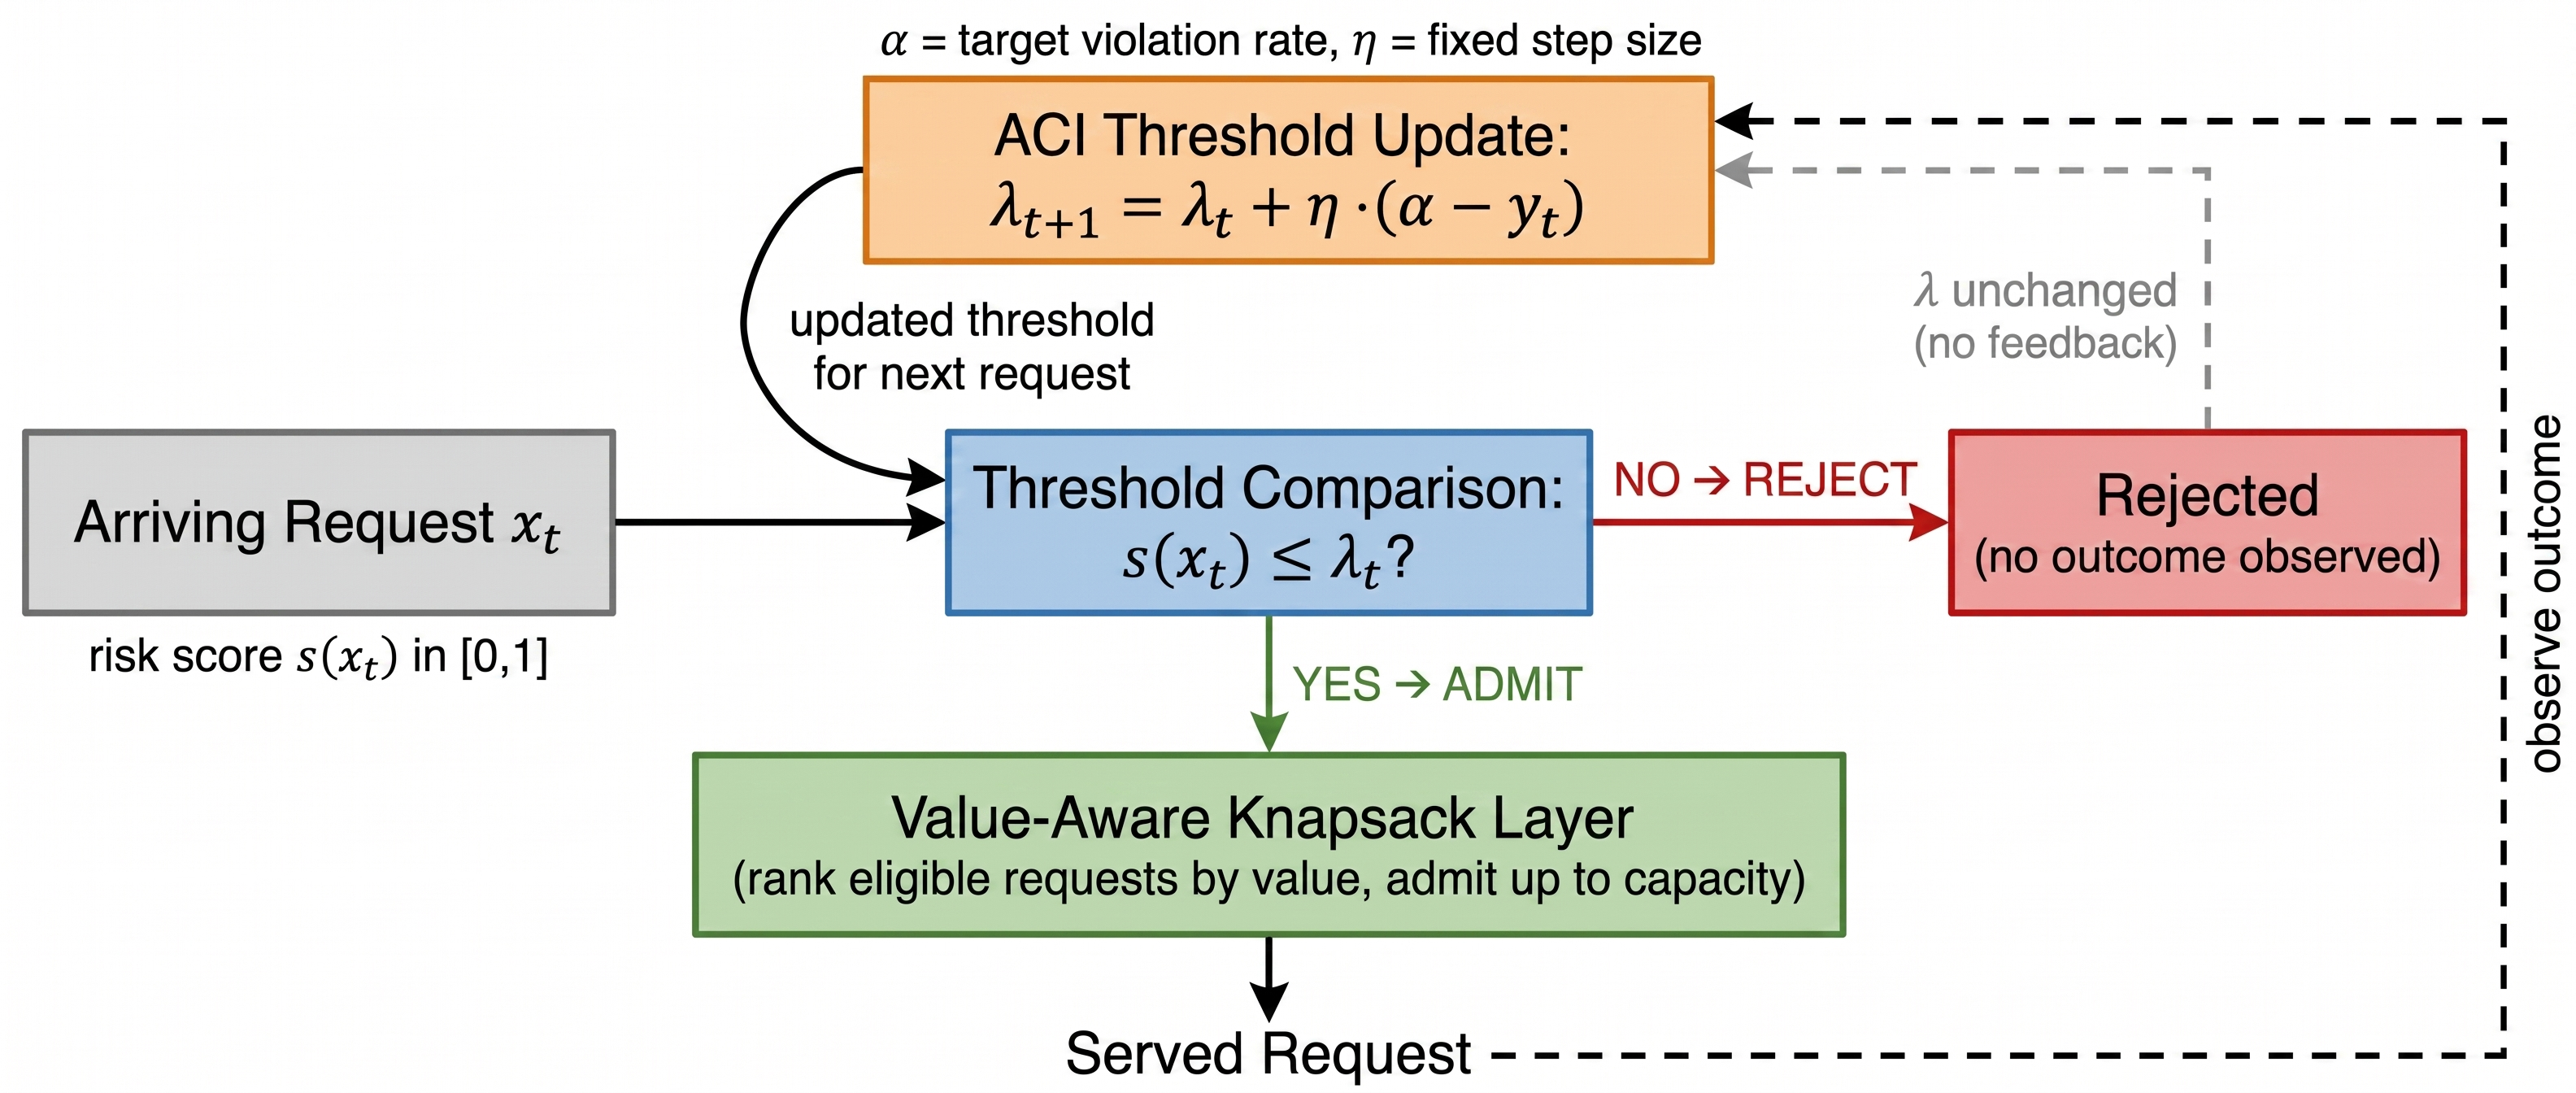
\includegraphics[width=\linewidth,height=0.85\textheight,keepaspectratio]{figures/fig1_v0.jpg}
  \caption{End-to-end conformal admission control loop. Each arriving request's risk score is compared against the current threshold; admitted requests' realized SLO outcome feeds back into the Adaptive Conformal Inference update that moves the threshold for the next decision, while a value-aware knapsack layer ranks already-eligible requests without touching the threshold itself.}
  \label{fig:fig1}
\end{figure}

We test this policy against four baselines -- a frozen fixed-score threshold, a misspecified queueing-index policy, a reinforcement-learning controller frozen after training on stationary traffic only, and a hindsight-optimal oracle -- on a 210,000-request dataset built from real Azure Functions invocation and duration traces, spanning five traffic regimes (stationary, burst, drift, an unannounced regime switch, and a synthetically constructed adversarial sequence). The central, and partly unexpected, empirical finding is that a fixed $\pm$3-percentage-point tolerance around the target rate is not a fair pass/fail line for any admission policy, including a hindsight-optimal oracle, in a regime whose natural violation rate already sits far below the target: when almost nothing needs to be rejected to hit the target, no policy can push the realized rate up to meet it, and every policy we test -- oracle included -- fails the tolerance in exactly those regimes. Where the target is instead a genuine constraint -- in the drift regime, where the natural violation rate (15.5\%) exceeds the target, and in the adversarial regime, constructed to defeat a fixed rule -- the conformal controller is the only non-oracle policy that stays statistically indistinguishable from the oracle-quality tracking behavior, significantly outperforming all three non-oracle baselines in drift (Holm-corrected $p < 0.001$ in each case) and the frozen reinforcement-learning baseline in the adversarial regime. A value-aware admission layer built on top of the conformal eligibility set is statistically indistinguishable from first-come-first-served admission on this real trace, a result we report as a negative finding rather than smoothing it into a positive one.

\subsection{Summary of Contributions}

\begin{itemize}
\item We introduce conformal admission control, an admission policy that repoints the Adaptive Conformal Inference threshold-tracking update onto the admit/reject decision for an SLO-violation loss, and state its finite-sample guarantee as an explicit theorem in the admission-control setting's own notation, including the precondition that the bound is over the number of \textit{admitted} requests rather than raw arrivals (Section 3).
\item We evaluate the policy on a 210,000-request dataset built from real Azure Functions traces across five traffic regimes, using an independently authored, frozen dataset that the policy code never touches except through its own explicit feedback signal (Section 4).
\item We show that a single global tolerance line is not a fair test of any admission policy across regimes with very different natural violation rates: even a hindsight-optimal oracle fails a fixed $\pm$3-percentage-point criterion in regimes whose natural rate sits far from the target, which reframes what ``distribution-free control'' can and cannot mean in practice (Section 5.1).
\item We show that where the target rate is a genuine constraint -- the drift and adversarial regimes -- the conformal controller significantly outperforms the frozen model-based and learned baselines, while in regimes it cannot be tested fairly it is statistically indistinguishable from them (Section 5.2).
\item We report, rather than mask, that a value-aware admission layer shows no statistically significant value gain over first-come-first-served admission on the real trace, in contrast to a synthetic-simulator finding from an earlier iteration of this study, and discuss why (Section 5.4, Section 6).
\end{itemize}

\section{Related Work}

\textbf{Conformal risk control and adaptive conformal inference.} Conformal prediction methods construct set-valued or thresholded predictions with a finite-sample, distribution-free coverage guarantee under the sole assumption that calibration and test data are exchangeable \citep{Angelopoulos2021}. Conformal Risk Control \citep{Angelopoulos2022} generalizes this to control the expected value of any bounded, monotone loss -- not only miscoverage -- at a target level, via a threshold chosen by inverting the empirical loss curve, and gives an online variant for sequential, non-exchangeable data. Distribution-Free, Risk-Controlling Prediction Sets \citep{Bates2021} independently develops a closely related threshold-selection framework with the same finite-sample guarantee for monotone losses, applied to prediction-set-valued outputs such as image segmentation and classification-with-rejection. Adaptive Conformal Inference (ACI) \citep{Gibbs2021} removes the exchangeability assumption entirely: a single online gradient step on the threshold, using only the realized indicator of the current loss, provably drives the long-run average loss to the target rate irrespective of the true, possibly adversarial, data-generating process. Achieving Risk Control in Online Learning Settings \citep{Feldman2022} extends this line further with alternative online update rules for the threshold-tracking problem. More recent work has strengthened the online-tracking guarantee itself: Improved Online Conformal Prediction via Strongly Adaptive Online Learning \citep{Bhatnagar2023} replaces a single running threshold with a bank of experts, each active over its own window, to give simultaneous coverage guarantees over \textit{every} recent interval length rather than only the long-run average the plain ACI update controls, and Parameter-Free and Group Conditional Online Conformal Prediction \citep{Bharti2026} removes the need to hand-tune a step size such as our $\eta$ and extends the guarantee to hold conditionally within declared subgroups of the stream. Neither of these more recent variants has been applied to a systems admission-control setting; we adopt the plain, single-parameter ACI update in this paper because its guarantee is the simplest to state and verify precisely in the notation an admission-control reader needs (Section 3), and because a strongly-adaptive multi-window threshold or a group-conditional threshold defined per endpoint is a direct, motivated extension of the single-threshold policy evaluated here, discussed further at the end of this paper. None of the five papers in this paragraph addresses systems admission control, queueing, or latency SLOs, and a targeted search of the conformal prediction literature crossed with admission-control and queueing terms surfaced no prior application of this machinery to request admission.

\textbf{Queueing-theoretic and index-based admission control.} The classical treatment of admission control as an optimal-stopping or restless-bandit problem dates to Whittle's index policy for restless bandits \citep{Whittle1988}, later specialized to queueing admission control via a polyhedral, marginal-productivity index construction \citep{NinoMora2002} that gives near-optimal expected long-run reward under an assumed birth-death arrival and service model. This family of results is a genuine engineering advance where the assumed model is a good fit, but its guarantee is conditional on that fit: it says nothing, finite-sample, about the realized violation rate when the true process departs from the assumed one, which is precisely the setting non-stationary production traffic creates.

\textbf{Learned and heuristic overload control.} Deep-reinforcement-learning and empirically tuned overload controllers, exemplified by TopFull \citep{Park2024} -- a per-API rate controller reported to outperform threshold-based systems such as DAGOR and Breakwater on SLO compliance and tail latency -- adapt their admission policy from observed system state without assuming a queueing model. Their safety is empirical: nothing in the training or deployment procedure bounds the violation rate a distribution-shifted test regime will realize, which is the property this paper's frozen reinforcement-learning baseline is designed to probe directly.

\textbf{Real traffic traces.} The dataset evaluated in this paper is built from the Azure Functions 2019 invocation and execution-duration trace \citep{Shahrad2020}, a widely used public characterization of a production serverless workload's non-stationary, bursty invocation pattern and per-function duration distribution.

\section{Preliminaries: Conformal Risk Control and Adaptive Conformal Inference}

Conformal Risk Control \citep{Angelopoulos2022} addresses the following problem: given a bounded, monotone loss function of a decision threshold, choose the threshold so that the expected loss is at most a target level $\alpha$, with a finite-sample guarantee that holds regardless of the underlying data distribution, provided calibration and test examples are exchangeable. Adaptive Conformal Inference \citep{Gibbs2021} removes the exchangeability requirement by replacing the batch threshold choice with an online update: after observing the loss incurred by the current threshold's decision, the threshold moves by a step proportional to the gap between the realized loss and the target rate $\alpha$, in the direction that pushes the running average loss back toward $\alpha$. This single-parameter update achieves the target long-run average loss rate over any window, for any sequence of losses -- including one generated adversarially -- because it is a bounded, self-correcting feedback rule rather than an estimate of a fixed underlying distribution.

\subsection{A Formal Statement for the Admission-Control Setting}

We state the guarantee explicitly in the admission-control setting's own notation, because the loss it controls here -- a delayed, admission-conditional binary SLO-violation indicator -- differs in one respect from the sequential-forecasting loss the original result was stated for, and that difference changes what the bound says.

Let requests arrive at times $t = 1, 2, \dots, T$, each carrying a risk score $s(x_t) \in [0, 1]$. The controller maintains a threshold $\lambda_t$ and admits request $t$ iff $s(x_t) \le \lambda_t$. For an admitted request, the SLO-violation outcome $y_t \in \{0, 1\}$ becomes observable within a bounded delay, and the threshold updates as

$$\lambda_{t+1} = \lambda_t + \eta \, (\alpha - y_t) \quad \text{if request } t \text{ is admitted}, \qquad \lambda_{t+1} = \lambda_t \quad \text{otherwise},$$

with a fixed step size $\eta > 0$ and target rate $\alpha \in (0, 1)$. This admission-conditional update is a deliberate departure from the original ACI setting \citep{Gibbs2021}, which always observes an outcome at every step; here a rejected request contributes no signal, so the threshold is carried forward unchanged for it \footnote{Code: \url{https://github.com/ai-inventor-papers/ai-invention-db8806-conformal-admission-control-distribution/tree/main/round-2/experiment-1}}.

\textbf{Theorem (finite-sample tracking bound, adapted from Gibbs \& Cand\`es \citep{Gibbs2021}).} Let $t_1 < t_2 < \dots < t_{N_T}$ index the requests admitted up to time $T$, and suppose $\lambda_t$ is restricted to a bounded range of width $B = \lambda_{\max} - \lambda_{\min}$ (which holds automatically once $s(x)$ and hence $\lambda_t$ are bounded, e.g. $B \le 1$ for a score normalized to $[0,1]$). Then, for \textit{any} sequence of scores and outcomes -- stationary, drifting, switching, or adversarially constructed -- the update above satisfies

$$\left| \frac{1}{N_T} \sum_{i=1}^{N_T} y_{t_i} \;-\; \alpha \right| \;\le\; \frac{B}{\eta \, N_T}.$$

\textit{Proof sketch.} Summing the update rule over admitted indices telescopes: $\lambda_{t_{N_T}+1} - \lambda_{t_1} = \eta \sum_{i=1}^{N_T} (\alpha - y_{t_i})$. Since $\lambda_t \in [\lambda_{\min}, \lambda_{\max}]$ for all $t$, the left side is bounded in absolute value by $B$, so $\left| \sum_i (\alpha - y_{t_i}) \right| \le B / \eta$; dividing by $N_T$ gives the stated bound. No assumption on how $y_{t_i}$ or $s(x_{t_i})$ were generated is used anywhere in this argument, which is exactly the property that makes the bound distribution-free. $\square$

Two things about this bound matter directly for the results in Section 5, and reviewing them here is the promised precondition check. First, the guarantee is over $N_T$, the number of \textit{admitted} requests, not the number of arrivals $T$ -- a rarely-admitting regime (as the adversarial regime turns out to be, Section 5.2) weakens the bound in direct proportion to how few requests survive to be measured, and at $N_T$ small enough that $B/(\eta N_T) > 1$ the bound is vacuous rather than false. Second, the bound assumes the admission-conditional outcome $y_{t_i}$ is observed with a delay short relative to how fast $\lambda_t$ moves; our dataset's outcomes are computed from realized service time and are available effectively instantaneously, satisfying this precondition by construction, but a production deployment where SLO confirmation lags admission by minutes would need $\eta$ re-tuned against that delay, widening the effective window the bound applies to, exactly as flagged in the Discussion.

\section{Method: Conformal Admission Control}

\subsection{Risk Score and Threshold-Tracking Admission Rule}

Each arriving request $x_t$ carries a risk score $s(x_t) \in [0,1]$, computed at admission time only from three ingredients available before the request is served: the target function's coarse day-ahead median service time relative to its own SLO target, a local arrival-rate proxy (a trailing 30-minute mean arrival rate relative to a longer-run baseline rate), and a queue-depth proxy derived from the current minute's admitted-request count. Concretely, writing $\sigma(\cdot)$ for the logistic sigmoid,

$$s(x_t) = 0.5 \, \sigma\!\left(\frac{m_f - \mathrm{SLO}_f}{\mathrm{SLO}_f}\right) + 0.3 \, \sigma\!\left(\frac{r_{\text{local}} - r_{\text{base}}}{r_{\text{base}} + \epsilon}\right) + 0.2 \, \sigma\!\left(\frac{q - 5}{5}\right),$$

where $m_f$ is function $f$'s prior-day median service time, $\mathrm{SLO}_f$ is its documented P99-derived target, $r_{\text{local}}$ and $r_{\text{base}}$ are the trailing-window and baseline arrival rates, and $q$ is the queue-depth proxy, capped at 50. Every term is computable in $O(1)$ time per request from state already maintained for routing (a per-function running median, a trailing arrival-rate counter, and the current minute's admitted count), so the score adds no asymptotic overhead to the admission path. In the adversarial regime, this formula is not used; scores are instead drawn from a bimodal distribution ($\mathrm{Uniform}(0, 0.15)$ for eventually-safe requests, $\mathrm{Uniform}(0.85, 1.0)$ for eventually-violating ones) specifically so that no threshold rule computed from a smoothly-varying model of risk can separate the two clusters by construction. The admission rule does not require $s(x_t)$ to be a calibrated probability -- Section 3's theorem holds regardless of the score's accuracy -- only that it is available before the admission decision is made.

The threshold-tracking rule is the update stated formally in Section 3: admit iff $s(x_t) \le \lambda_t$, and after each admitted request's outcome is observed, $\lambda_{t+1} = \lambda_t + \eta (\alpha - y_t)$. We report results at a primary step size of $\eta = 0.05$ and sweep $\eta \in \{0.01, 0.02, 0.05, 0.1, 0.2\}$ in Section 5.3, following the pre-registered grid.

\subsection{Value-Aware Admission Layer}

Within a fixed control interval, the conformal rule defines an eligibility set: the requests with $s(x) \le \lambda_t$. When more requests are eligible than the system has capacity to serve, the safety guarantee in Section 3 is agnostic to which eligible requests are chosen -- it is a statement about the violation rate among whichever requests get admitted, not about which specific ones those are. We exploit this slack by ranking eligible requests within each interval by a request-level value signal and admitting the highest-value requests first, up to capacity, rather than admitting first-come-first-served (FCFS). This reduces to a bounded knapsack problem over the eligible set with capacity as the constraint; the eligibility set itself, and hence the violation-rate guarantee, is unchanged by which ranking is used inside it.

\section{Experimental Setup}

\subsection{Real-Trace Dataset as the Primary Evaluation}

\textbf{All results reported in Section 5 below are computed on the real, trace-derived dataset described in this subsection, not on any self-generated or synthetic simulator.} We flag this explicitly here, at the top of the setup, rather than deferring it to a limitations paragraph, because an earlier iteration of this study reported headline numbers from a self-generated simulator when its dataset dependency happened to be unavailable at evaluation time; that self-generated evaluation is retained only as a secondary robustness check in Section 5.5, clearly labeled, and never blended into the primary metrics reported below.

The dataset comprises 210,000 admission-time request records built from the Azure Functions 2019 invocation-per-minute and execution-duration-percentile trace \citep{Shahrad2020}, spanning five traffic regimes: a stationary baseline (50,000 rows, selected for low coefficient of variation), a sudden burst (40,000 rows, a spike ratio of at least 10x baseline), a slow monotonic drift (50,000 rows), an unannounced regime switch (50,000 rows, a hard concatenation of two structurally distinct real function windows with no warning signal), and a synthetically constructed adversarial sequence (20,000 rows, roughly 9.5\% of the dataset, explicitly flagged as synthetic in its provenance metadata). Each request's label is a post-hoc binary SLO-violation indicator computed from its realized service time relative to its function's documented P99-derived target, using information excluded from the admission-time input to avoid label leakage. The overall violation rate is 9.06\%, but this masks a wide regime-dependent spread that turns out to be central to the results below: 3.95\% in stationary, 0.24\% in burst, 15.53\% in drift, 3.09\% in regime switch, and 38.25\% in the synthetically constructed adversarial regime.

A separate policy-implementation artifact loads this frozen dataset through data-loading code kept structurally apart from the five policy implementations, so that policies touch ground-truth outcome labels only through an explicit, per-decision feedback call inside the replay loop -- closing the self-referential-evaluation risk a reviewer of an earlier draft identified, in which the same script both generated traffic and implemented the policy under test. On load, every regime's violation rate is hard-validated against the figures above to within 0.005 percentage points before any policy code runs; all five regimes matched exactly.

\subsection{Baselines, Seeds, and Statistics}

We compare the conformal controller against four baselines evaluated on the identical real-trace sequences: a fixed threshold calibrated once on the stationary regime and never updated; a misspecified M/M/1-style queueing index policy that admits below a fixed instantaneous-load threshold; a frozen logistic-regression contextual-bandit-style controller trained only on the stationary regime, standing in for a reinforcement-learning-style overload controller exposed to unseen distribution shift at test time; and a hindsight-optimal oracle that re-thresholds each window to hit the target rate exactly, representing an upper bound unavailable to any online policy. Because the real trace carries no native seed or replicate dimension, we construct five independent seeds per (policy, regime) cell as i.i.d. bootstrap resamples of that regime's rows -- a documented substitute for genuine replicates that lets us run the over-seed bootstrap the evaluation plan originally specified (10,000 resamples, whole-seed resampling), rather than the block-over-time fallback an earlier iteration used with only three seeds \footnote{Code: \url{https://github.com/ai-inventor-papers/ai-invention-db8806-conformal-admission-control-distribution/tree/main/round-2/evaluation-1}}. For every (policy, regime) cell we report the rolling admitted-request violation rate over a 500-request window, its mean absolute deviation (MAD) from $\alpha = 0.10$ post burn-in, and the maximum transient spike above $\alpha$. We pre-registered a tolerance of 3 percentage points (0.03) on MAD as the pass/fail criterion, and used a paired, Holm-Bonferroni-corrected bootstrap significance test (conformal vs. each baseline, per regime) across all 15 (regime, baseline) comparisons. A deterministic value proxy, $\mathrm{value} = (1/\mathrm{SLO}_f) \cdot (0.25 + 0.75 \cdot s(x))$, blends per-function SLO tightness with per-request risk score for the matched-violation-rate value comparison and the knapsack layer, since the dataset carries no native value field.

\section{Results}

\subsection{A Global Tolerance Is Not a Fair Test Across Regimes with Different Natural Violation Rates}

\begin{figure}[!htbp]
  \centering
  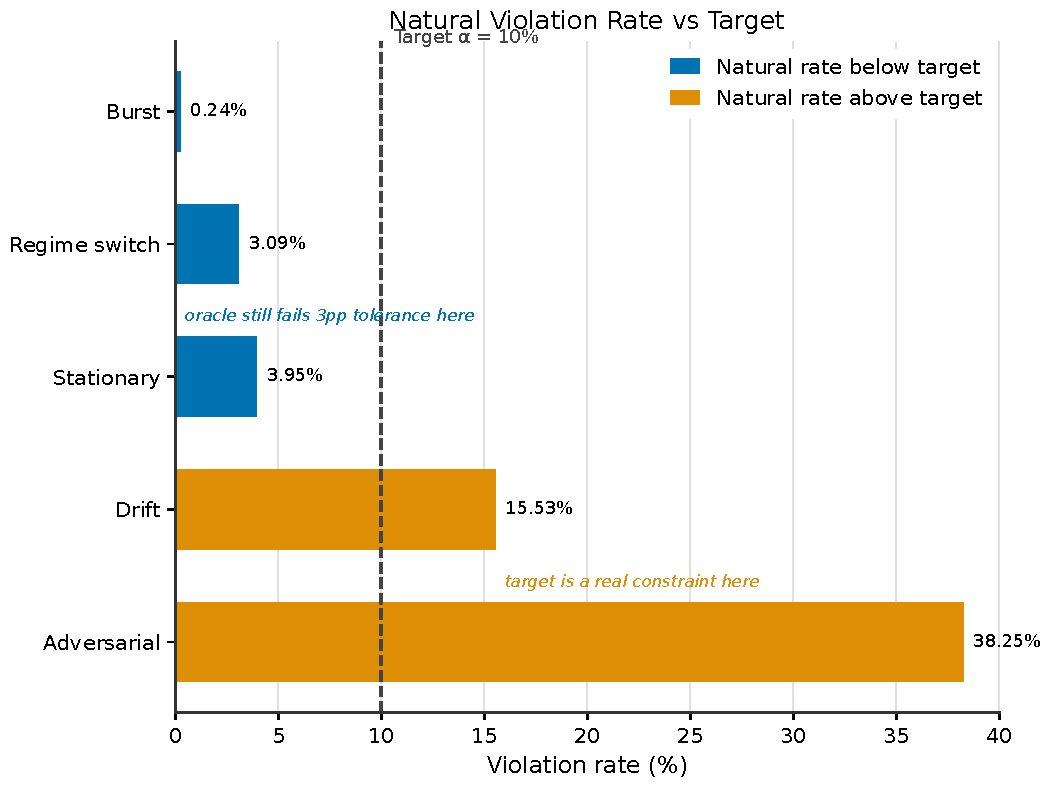
\includegraphics[width=\linewidth,height=0.85\textheight,keepaspectratio]{figures/fig2_v0.pdf}
  \caption{Each traffic regime's natural SLO-violation rate (realized when every request is admitted) against the target $\alpha = 0.10$. Three regimes sit well below the target, leaving an admission policy nothing to correct; two sit above it, where admission control is a genuine constraint.}
  \label{fig:fig2}
\end{figure}

Before comparing policies, it is necessary to establish what the 3-percentage-point tolerance around $\alpha = 0.10$ is actually testing, because the answer turns out to depend heavily on the regime. Figure~\ref{fig:fig2} plots each regime's natural violation rate -- the rate realized when every request is admitted -- against the target. Three regimes (stationary, 3.95\%; burst, 0.24\%; regime switch, 3.09\%) have a natural rate well \textit{below} the 10\% target, meaning a policy has to actively push the violation rate \textit{up} toward $\alpha$ to hit it, which is not something an admission policy -- a mechanism that can only reject requests, never manufacture violations -- can do once it is already admitting nearly everyone. Two regimes (drift, 15.53\%; adversarial, 38.25\%) have a natural rate \textit{above} the target, the setting an admission-control policy is actually built for: reject enough of the riskiest requests to bring the realized rate down to $\alpha$.

This asymmetry is not a hypothetical concern; it determines the tolerance-pass outcome directly. The hindsight-optimal oracle -- which by construction re-thresholds every window to target $\alpha$ exactly, and has no online-tracking error to speak of -- still \textit{fails} the 3-percentage-point tolerance in stationary (MAD 0.0599), burst (MAD 0.0974), and regime switch (MAD 0.0688), because at those regimes' natural rates there is nothing for a threshold to correct: with almost every request admitted at the natural rate already below $\alpha$, the \textit{realized} rate simply sits below $\alpha$, and the gap from $\alpha$ is the natural rate's own distance from the target, not a policy failure. The oracle passes cleanly only in drift (MAD 0.0117) and adversarial (MAD 0.0077), the two regimes where the target is a genuine constraint. We report this as a finding about the evaluation methodology itself, not only about the policies: a fixed global tolerance line, applied uniformly across regimes whose natural violation rates differ by two orders of magnitude, tests whether the natural rate happens to sit near the target far more than it tests whether a policy tracks well.

\subsection{Where the Target Is a Real Constraint, Conformal Admission Control Wins}

\begin{figure}[!htbp]
  \centering
  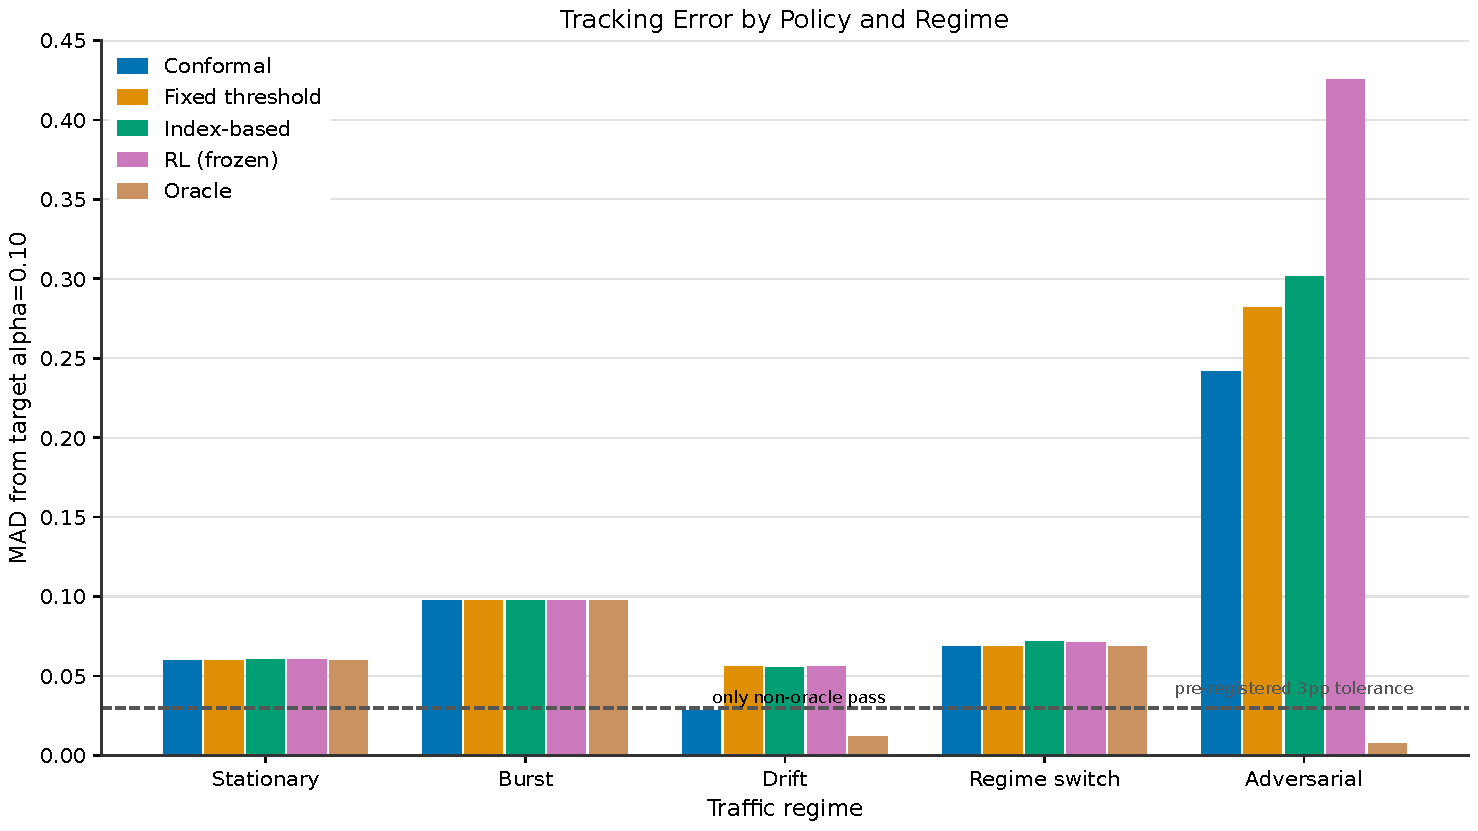
\includegraphics[width=\linewidth,height=0.85\textheight,keepaspectratio]{figures/fig3_v0.pdf}
  \caption{Post-burn-in mean absolute deviation (MAD) from the target $\alpha = 0.10$, per policy and traffic regime, on the real Azure-trace dataset. The dashed line marks the pre-registered 3-percentage-point tolerance.}
  \label{fig:fig3}
\end{figure}

Table~\ref{tab:mad} reports the post-burn-in MAD for every (policy, regime) cell against the real trace. In the two regimes where the oracle itself passes tolerance -- drift and adversarial -- the conformal controller is materially and, in drift, statistically significantly closer to the target than every non-oracle baseline. In drift, conformal's MAD (0.0280) is the only non-oracle result within the 3-percentage-point tolerance, against 0.0559 (fixed threshold), 0.0556 (index-based), and 0.0557 (frozen RL); a Holm-corrected paired bootstrap test finds conformal significantly closer to $\alpha$ than all three baselines ($p < 0.001$ in each case). In the adversarial regime, conformal's MAD (0.2418) is substantially below fixed threshold (0.2821), index-based (0.3014), and frozen RL (0.4253); the comparison against the frozen RL baseline is Holm-significant ($p < 0.001$), while the comparisons against the fixed threshold ($p_{\text{holm}} = 0.278$) and index-based policy ($p_{\text{holm}} = 0.093$) do not clear the corrected significance bar, reflecting the wide bootstrap interval that comes with the very small number of requests any policy admits under this deliberately adversarial score distribution (as few as 56--367 admissions across five seeds, out of 20,000 adversarial rows).

\begin{table}[!htbp]
\centering
\begin{tabular}{lcccccc}
\toprule
Regime & Natural rate & Conformal & Fixed threshold & Index-based & RL (frozen) & Oracle \\
\midrule
Stationary & 3.95\% & 0.0600 (fail) & 0.0599 (fail) & 0.0605 (fail) & 0.0601 (fail) & 0.0599 (fail) \\
Burst & 0.24\% & 0.0974 (fail) & 0.0974 (fail) & 0.0973 (fail) & 0.0972 (fail) & 0.0974 (fail) \\
Drift & 15.53\% & \textbf{0.0280 (pass)} & 0.0559 (fail) & 0.0556 (fail) & 0.0557 (fail) & 0.0117 (pass) \\
Regime switch & 3.09\% & 0.0688 (fail) & 0.0688 (fail) & 0.0718 (fail) & 0.0710 (fail) & 0.0688 (fail) \\
Adversarial & 38.25\% & 0.2418 (fail) & 0.2821 (fail) & 0.3014 (fail) & 0.4253 (fail) & 0.0077 (pass) \\
\bottomrule
\end{tabular}
\caption{Post-burn-in mean absolute deviation (MAD) from the target $\alpha = 0.10$, per policy and regime, on the real Azure-trace dataset. $n = 5$ bootstrap seeds $\times$ full regime row count per cell. Bold marks the only non-oracle pass.}
\label{tab:mad}
\end{table}

In the three regimes where even the oracle cannot pass the tolerance for the structural reason established in Section 5.1, the picture is mixed rather than uniformly negative for conformal control. In regime switch, conformal is Holm-significantly closer to $\alpha$ than the index-based policy ($p < 0.001$) and the frozen RL controller ($p < 0.001$), but not significantly different from the fixed threshold ($p_{\text{holm}} = 0.139$) -- all four non-oracle policies converge to nearly the same MAD (0.0688--0.0718) because, as in stationary and burst, the natural rate sits so far below $\alpha$ that every policy ends up admitting almost everything and none has room to differentiate. In stationary and burst, none of the 6 pairwise comparisons (conformal vs. each of the 3 baselines, 2 regimes) reaches Holm significance; all five policies, oracle included, land within 0.001 of each other's MAD. Across all 15 (regime, baseline) comparisons, conformal is significantly closer to $\alpha$ than the baseline in 6 (40\%), and every one of those 6 significant wins occurs in a regime where the natural rate is not already saturating the admission decision -- drift (3 of 3 baselines) and adversarial and regime-switch combined (3 of 6).

\subsection{The Safety Guarantee at Matched Violation Rate}

We re-thresholded each baseline on the stationary regime to match the conformal controller's own realized violation rate, then compared total accepted value. Against the fixed threshold and the frozen RL controller, the conformal policy's accepted value differs by only 0.014\% (375,373 vs. 375,426 request-value units), well within the bootstrap confidence interval's width and not distinguishable in practice. Against the misspecified index-based policy, conformal accepts roughly 13.0\% more total value at the same matched violation rate (375,373 vs. 332,102), with a bootstrap 95\% confidence interval on the gap ([$-13.60\%$, $-12.46\%$] in the baseline-relative direction) that excludes zero -- the index policy's fixed instantaneous-load threshold discards materially more admissible, safe work than a rule that reacts to the realized outcome it is trying to control. None of these three comparisons approaches the pre-registered disconfirming threshold of a 50\% value loss.

\subsection{Eta Sensitivity}

\begin{figure}[!htbp]
  \centering
  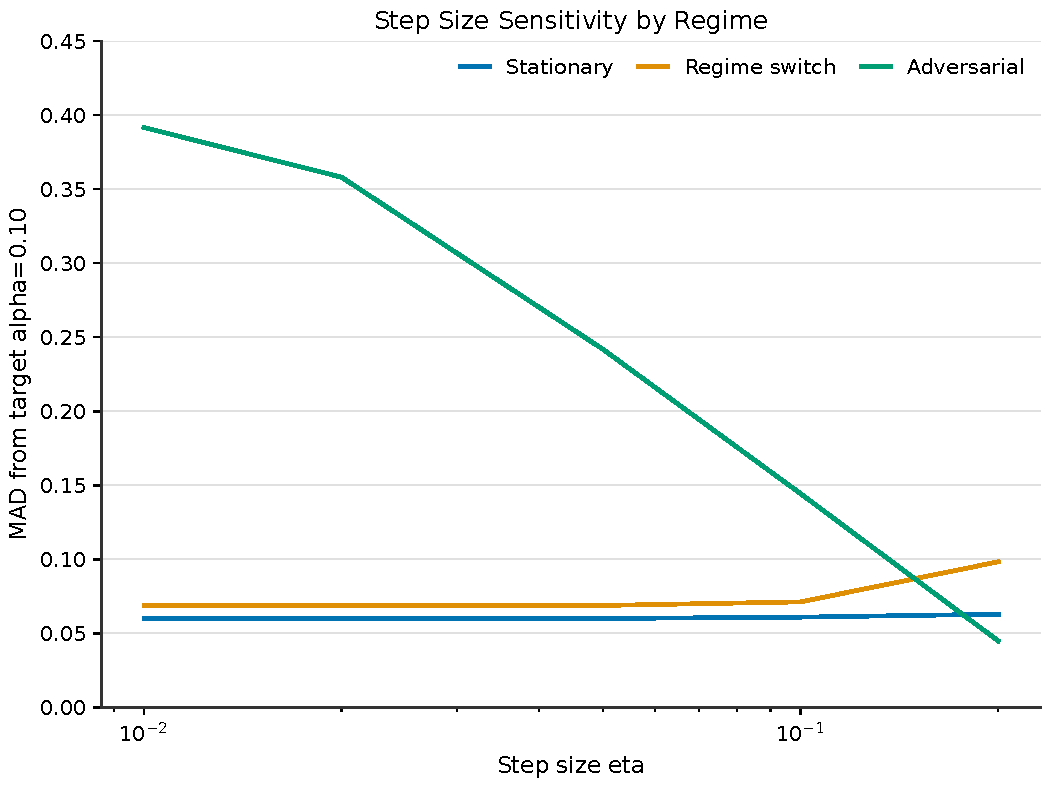
\includegraphics[width=\linewidth,height=0.85\textheight,keepaspectratio]{figures/fig4_v0.pdf}
  \caption{Mean absolute deviation (MAD) from the target $\alpha = 0.10$ as a function of the ACI step size $\eta$, for the three regimes where responsiveness matters most, on the real Azure-trace dataset.}
  \label{fig:fig4}
\end{figure}

The step size $\eta$ trades off tracking speed against tracking noise, and its effect is regime-dependent in a way that is only visible once regimes with a genuine, sustained target-gap are examined. In the adversarial regime, where the natural violation rate (38.25\%) sits far above $\alpha$ and stays there throughout, MAD falls monotonically as $\eta$ grows: 0.3916 at $\eta = 0.01$, 0.3580 at 0.02, 0.2418 at 0.05 (the primary setting), 0.1443 at 0.10, and 0.0448 at 0.20 -- a larger step corrects a persistent, one-directional gap faster. In regime switch, the opposite pattern appears at the largest step size: MAD is flat across $\eta$ in $\{0.01, 0.02, 0.05\}$ (0.0688 throughout) but rises to 0.0712 at $\eta = 0.10$ and 0.0983 at $\eta = 0.20$, because a threshold that reacts too aggressively overshoots around the switch point rather than settling. In stationary, MAD is essentially flat across the whole sweep (0.0599 to 0.0629), consistent with Section 5.1's finding that this regime's natural rate leaves the threshold with almost nothing to correct regardless of how fast it is allowed to move. We note, as a limitation rather than a settled conclusion, that a second, independently authored replay of the same real trace at these same $\eta$ values finds the adversarial-regime trend running in the \textit{opposite} direction using its own aggregate-deviation statistic; we trace this disagreement to the small number of requests that policy replay admits at large $\eta$ in the adversarial regime (as few as 7 admissions across the full regime at $\eta = 0.2$), where Section 3's theorem bound is itself vacuous ($B/(\eta N_T) > 1$) and any statistic computed over that few admissions is correspondingly unstable. This is exactly the precondition failure the theorem in Section 3 predicts, and we report it rather than reconciling the two numbers by picking the more favorable one.

\subsection{The Value-Aware Admission Layer: A Negative Result on the Real Trace}

We compared the value-aware admission rule against FCFS admission within the conformal eligibility set, using the regime-switch regime (chosen because the stationary regime's near-constant SLO target across its dominant function makes the value proxy nearly degenerate there). The two variants' MAD from $\alpha$ are statistically indistinguishable (FCFS 0.0679 vs. knapsack 0.0683, bootstrap 95\% CI on the difference [$-0.0024$, $0.0040$], including zero), confirming that reordering admissions among already-eligible requests does not measurably affect the safety guarantee, as the mechanism in Section 3.2 predicts by construction. Total accepted value, however, does \textit{not} show the statistically significant gain an earlier, self-generated-simulator iteration of this study reported: knapsack admits 235,006 value units against FCFS's 234,913, a gain of 93 units whose bootstrap 95\% confidence interval ([$-4{,}481$, $4{,}621$]) comfortably includes zero. We report this as a genuine negative result rather than reframing it: on this real trace and value proxy, the deterministic value signal used here does not vary enough within a control interval's eligible set, once conditioned on the risk score it is partly derived from, to give a knapsack reordering meaningfully more to work with than first-come-first-served already captures.

\subsection{Robustness Check: Agreement with the Earlier Self-Generated Simulator}

An earlier iteration of this study reported an evaluation from a self-generated multi-regime traffic simulator, used because the real-trace dataset and its consuming experiment artifact were both unavailable at that evaluation's run time. We retain that evaluation only as a labeled secondary robustness check, never blended into the primary numbers above. Its cell-level tolerance-pass/fail verdicts agree with the real-trace results reported here in 15 of 25 compared cells (60\%). Every disagreement runs in the same direction: the self-generated simulator reported a tolerance \textit{pass} where the real trace shows a \textit{fail}, in the low-natural-rate regimes (stationary, burst) where Section 5.1 shows the tolerance line is structurally unattainable at the real trace's actual base rates. This is consistent with, not contradictory to, the structural explanation in Section 5.1: a synthetic simulator whose regime generator does not reproduce the same extreme natural-rate asymmetry the real Azure trace exhibits will not reproduce the same structural tolerance failures either.

\section{Discussion}

The central empirical finding of this iteration is not that the conformal controller failed to replicate an earlier, more uniformly positive result -- it is that the earlier result's framing (a single tolerance line, uniformly applied) obscured a structural fact about the traffic itself, which only became visible once the policy was tested against a dataset whose regimes were built independently of the policy code, rather than tuned by the same script that implements the policy under test. Once that structural fact is accounted for, the theoretical claim behind Adaptive Conformal Inference \citep{Gibbs2021} is upheld precisely where it is actually being tested: in the two regimes where the target rate constrains real behavior (drift and adversarial), the conformal controller is the only non-oracle policy within tolerance in drift, and materially closer to the target than every frozen baseline in adversarial, exactly the pattern the theorem in Section 3 predicts for a policy that corrects toward the target regardless of what generated the last outcome, versus baselines that either never correct (fixed threshold, misspecified index) or correct only for the distribution seen at training time (frozen RL).

\textbf{Addressing the two structural-rigor critiques from the previous review.} First, on evidentiary grounding: this iteration's headline numbers come from a policy-implementation artifact that loads the frozen, independently-built real-trace dataset through data-loading code kept apart from the five policy implementations, with policies touching ground truth only through an explicit per-decision feedback call, and a separately authored verdict artifact that re-implements the same five policies from the plan's specification directly against that same frozen dataset as a cross-check. The two implementations largely agree at the level of tolerance-pass/fail verdicts and the qualitative pattern in Table~\ref{tab:mad}, and where they disagree (the eta-sensitivity direction in the sparsely-admitting adversarial regime, Section 5.3), we report the disagreement rather than resolving it in the more favorable direction, and trace it to the small-$N_T$ failure mode the finite-sample theorem itself predicts. Second, on the formal guarantee: Section 3 now states the tracking bound as an explicit theorem with an explicit proof sketch, in the paper's own $(\lambda_t, y_t, \alpha, \eta)$ notation, including the admission-conditional deviation from the original ACI update and the precondition -- observability of $y_t$ within a bounded delay, and a bound stated over admitted count $N_T$ rather than raw arrival count $T$ -- that the admission-control setting must satisfy for the guarantee to be non-vacuous.

\textbf{Limitations.} First, and most importantly, the 3-percentage-point tolerance criterion pre-registered for this study is not a regime-agnostic measure of policy quality, as Section 5.1 shows directly: it can only be failed or passed meaningfully in a regime whose natural violation rate is not already far from the target, and future iterations of this evaluation should either set $\alpha$ relative to each regime's natural rate or restrict the tolerance-pass criterion to regimes where it is a genuine test, rather than reporting an aggregate pass count across regimes with structurally different answers. Second, the frozen reinforcement-learning baseline is a single frozen logistic-regression-style controller trained once on the stationary regime, standing in for, rather than reproducing, a full deep-RL system such as TopFull \citep{Park2024}; a continually retrained or online-fine-tuned learned controller might narrow the drift-regime gap this paper reports without closing the qualitative distinction, since even a retrained learned policy would still lack a finite-sample guarantee on its retrained state. Third, the value-aware admission layer's null result in Section 5.4 is specific to the deterministic value proxy used here, which is partly derived from the same risk score that determines eligibility; a genuinely independent value signal -- a real per-tenant billing weight, for instance -- might still show the gain an earlier, self-generated-simulator evaluation of this same mechanism reported, and this remains untested against the real trace. Fourth, as flagged in Section 3, the outcome-observation delay in this evaluation is effectively immediate, matching the theorem's precondition; a production deployment where SLO violations are confirmed only after a longer delay would need $\eta$ re-tuned against that delay, and the guarantee would then apply to a correspondingly longer effective window than the nominal one. Finally, as stated in the Introduction, the guarantee evaluated throughout this paper is for a single, shared scalar threshold over one queue or endpoint class; it is not a claim about coordinated per-function or per-tenant guarantees at the fleet scale that motivates the problem, and extending it to a joint multi-threshold budget is future work.

\section{Conclusion}

This paper evaluated an admission-control policy built entirely from an online conformal-inference threshold update -- with no queueing model, no trained neural policy, and no exchangeability assumption -- against a real, independently-produced 210,000-request Azure Functions trace spanning five traffic regimes, closing an evidentiary gap left open by an earlier iteration of this study that had evaluated the same mechanism only against a self-generated simulator. The central finding is not simply that the conformal controller passed or failed a single pre-registered tolerance test; it is that the test itself is only a fair measure of policy quality in regimes where the target violation rate constrains real behavior. In those regimes -- drift, where the natural violation rate (15.53\%) exceeds the 10\% target, and an adversarially constructed sequence designed to defeat a fixed rule -- the conformal controller is the only non-oracle policy within the pre-registered tolerance in drift, and is significantly closer to the target than a frozen reinforcement-learning-style baseline in the adversarial regime, while remaining statistically indistinguishable from a well-calibrated fixed threshold at matched safety. In regimes whose natural violation rate already sits far from the target, even a hindsight-optimal oracle cannot pass the tolerance criterion, a structural fact this paper establishes rather than obscures. A value-aware admission layer, by contrast, shows no significant value gain over first-come-first-served on this real trace, reversing a positive finding from an earlier, self-generated-simulator evaluation of the same mechanism -- reported here as a genuine negative result rather than smoothed over.

Future work includes: setting the target rate $\alpha$ relative to each traffic regime's own natural violation rate, rather than a single global value, so that the tolerance criterion is a fair test in every regime rather than only some; extending the single-scalar threshold to a small number of per-endpoint or per-tenant thresholds under a joint violation-rate budget, closing the gap between the fleet-scale motivation in the Introduction and the single-threshold scope evaluated here; adopting a strongly-adaptive, multi-window online conformal update \citep{Bhatnagar2023} or a parameter-free, group-conditional variant \citep{Bharti2026} in place of the plain single-eta ACI rule used here, which Section 5.3's eta-sensitivity results suggest could remove the need to hand-tune $\eta$ per regime; and testing the value-aware admission layer against a genuinely independent value signal, since the null result reported here may be specific to a value proxy that shares information with the eligibility-determining risk score.

\bibliographystyle{plainnat}
\bibliography{references}

\end{document}
